\chapter{INTRODUCTION}
\label{chap:introduction}
\thispagestyle{fancy}
	
Special Note: Ensure that your thesis demonstrates a clear and realistic scope in terms of resources required, with a comprehensive contingency plan in place. Maintain a high level of clarity and coherence throughout the proposal by organizing the content logically and following a structured format. Pay meticulous attention to grammar, style, and language use, while also conducting thorough proofreading and editing to enhance the overall writing quality.

\section{Background}
\label{sec:background}
For your thesis introduction, keep it concise and clear. Start by explaining the background and why your research is important. State your research goal and mention the gap in existing knowledge. Present your thesis statement and mention any relevant concepts or theories, citing references as needed. Justify why your research problem matters and how it's novel. Ensure smooth transitions between ideas, maintain reader interest, and write in a well-structured and engaging manner, setting the stage for the rest of your work.

\begin{itemize}
	\item List 1
	\item List 2
	\item List 3
\end{itemize}

	\section{Problem Statement}
	\label{sec:problem-statement}
	In formulating a research problem, it is essential to identify a specific and well-defined issue within your field of study that warrants investigation. The research problem should be clear, concise, and compelling, posing a question or challenge that both contributes to the existing body of knowledge and has practical relevance. It should reflect a gap in current understanding, necessitating further exploration and analysis. A strong research problem serves as the foundation upon which your entire study is built, guiding the research process, and helping to define the scope and objectives of your research. To assist in defining research problems, a fishbone diagram is recommended.

	\begin{figure}[htbp]
		\centering 
		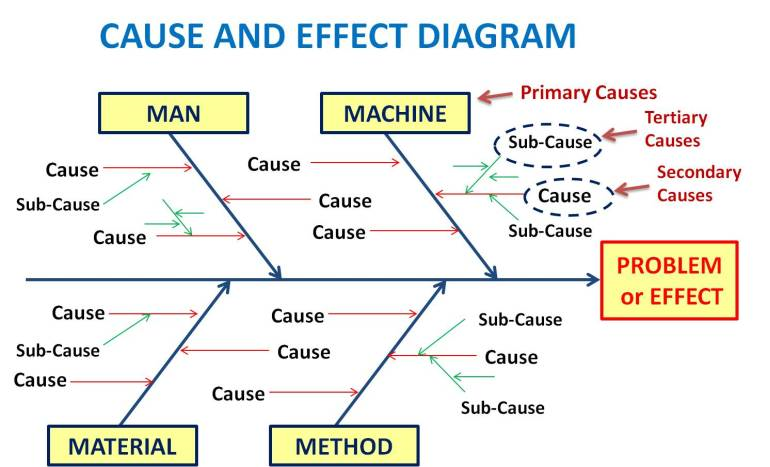
\includegraphics[width=0.8\textwidth]{images/fishbone.png}
		\caption{Example of fishbone diagram}
		\label{fig:fishbone}
	\end{figure} 

	Note: when you’re thinking about research problem and objective, please make sure your Feasibility, Realistic Timeline, Resource Availability, Data Availability, and Contingency Plan (Plan A, Plan B and Plan C with different scoping).

	\section{Research Objective}
	\label{sec:research-objective}	
	For Research Question and Objective, making sure they are specific and match the research problem. Ensure they can be measured and are feasible. Cover all aspects of the research objectives, problems, and gaps in a complete and coherent manner. Stay open to different approaches and maintain consistency throughout. Use clear and precise language while emphasizing the relevance and importance of your research. Keep in mind that each objective and question should be achievable within your research context. Overall, create a well-organized thesis that addresses each element of the assessment format effectively.
    
	\section{Research Question}
	\label{sec:research-question}
	For Research Question and Objective, making sure they are specific and match the research problem. Ensure they can be measured and are feasible. Cover all aspects of the research objectives, problems, and gaps in a complete and coherent manner. Stay open to different approaches and maintain consistency throughout. Use clear and precise language while emphasizing the relevance and importance of your research. Keep in mind that each objective and question should be achievable within your research context. Overall, create a well-organized thesis that addresses each element of the assessment format effectively.
    	
    \section{Hypothesis}
  	\label{sec:hypothesis}
		This is the body of your thesis. Please check that your body of thesis consistency in term of font type, font size, spacing, and margin are maintained. This is the body of your thesis. Please check that your body of thesis consistency in term of font type, font size, spacing, and margin are maintained.
	
	 \section{Research Scope and Limitation}
	  \label{sec:research-scope-of-works}
		This is the body of your thesis. Please check that your body of thesis consistency in term of font type, font size, spacing, and margin are maintained. This is the body of your thesis. Please check that your body of thesis consistency in term of font type, font size, spacing, and margin are maintained.

	\section{Significance of Study}
	\label{sec:significance-of-study}
	In this section you need to highlight or showcase the originality, methodological innovation, and practical implications for the field. Remember to emphasize the field relevance to the stakeholder, and the broader implications, while maintaining comprehensiveness and balance. Overall, your thesis should demonstrate how your work aligns with existing knowledge, contributes to theory and practice, and possesses the potential to reshape the field.

	\section{Thesis Structure}
	This is the body of your thesis. Please check that your body of thesis consistency in term of font type, font size, spacing, and margin are maintained. This is the body of your thesis. Please check that your body of thesis consistency in term of font type, font size, spacing, and margin are maintained.
    